\documentclass[a4paper,10pt]{article}
\usepackage[utf8]{inputenc}
\usepackage[spanish]{babel}
\usepackage[affil-it]{authblk}
\usepackage{enumerate}
\usepackage{graphicx}
\usepackage{hyperref}
\usepackage{amsmath}
\usepackage{amssymb}
\usepackage{cancel}
\usepackage{tikz}
\usepackage{float}
\usepackage{cleveref}
\usepackage[margin=1.4in]{geometry}
\usepackage[labelfont=bf]{caption}
\usetikzlibrary{calc}
\numberwithin{equation}{section}

%Indentation
\setlength{\parindent}{0ex}

%Multiple References

\usepackage{xparse}
\ExplSyntaxOn
\NewDocumentCommand{\mref}{m}{\quinn_mref:n {#1}}
\seq_new:N \l_quinn_mref_seq
\cs_new:Npn \quinn_mref:n #1
 {
  \seq_set_split:Nnn \l_quinn_mref_seq { , } { #1 }
  \seq_pop_right:NN \l_quinn_mref_seq \l_tmpa_tl
  ( % print the left parenthesis
  \seq_map_inline:Nn \l_quinn_mref_seq
    { \ref{##1},\nobreakspace } % print the first references
  \exp_args:NV \ref \l_tmpa_tl 
  ) 
 }
\ExplSyntaxOff


%Boxes

\newcommand*{\boxcolor}{blue}
\makeatletter
\renewcommand{\boxed}[1]{\textcolor{\boxcolor}{%
\tikz[baseline={([yshift=-1ex]current bounding box.center)}] \node [rectangle, minimum width=1ex,rounded corners,draw] {\normalcolor\m@th$\displaystyle#1$};}}
 \makeatother

%Constantes
\newcommand{\euler}{\mathrm{e}}
\newcommand{\im}{i}

%Lemas, teoremas, definiciones y pruebas
\newcommand{\definicion}{\textbf{Definición: }}
\newcommand{\lema}{\textbf{Lema: }}
\newcommand{\teorema}{\textbf{Teorema: }}
\newcommand{\prueba}{\textbf{Prueba: }}


%opening
\title{Mecánica Clásica Tarea \# 4}
\author{Favio Vázquez\thanks{Correo: favio.vazquezp@gmail.com}}\affil{Instituto de Ciencias Nucleares. Universidad Nacional Autónoma de México.}
\date{}

\begin{document}

\makeatletter
\def\@maketitle{%
  \newpage
  \null
  \vskip 2em%
  \begin{center}%
  \let \footnote \thanks
    {\Large\bfseries \@title \par}%
    \vskip 1.5em%
    {\normalsize
      \lineskip .5em%
      \begin{tabular}[t]{c}%
        \@author
      \end{tabular}\par}%
    \vskip 1em%
    {\normalsize \@date}%
  \end{center}%
  \par
  \vskip 1.5em}
\makeatother

\maketitle

\section{Problema 1}

Una partícula de masa $m_1$ se mueve a lo largo de una recta, otra de masa $m_2$ lo 
hace a lo largo de otra reta perpendicular a la primera. Las partículas interaccionan 
entre sí por medio de la gravedad. Encuentra las ecuaciones de movimiento. Usando 
una computadora trace una trayectoria en el espacio de configuración para algunas 
masas y condiciones iniciales.

\vspace{.3cm}

Suponga que $m_2=m_1+\epsilon$, donde $\epsilon$ es una cantidad pequeña. Encuentre 
las ecuaciones de movimiento a primer orden en $\epsilon$. Usando una computadora 
trace una órbita genérica para este caso.

\vspace{.3cm}

\underline{Solución:} \vspace{.3cm}


\section{Problema 2}

Encuentre las ecuaciones de movimiento del péndulo doble usando únicamente métodos 
vectoriales. El péndulo doble tiene las dos masas iguales y las dos longitudes iguales.
Usando una computadora trace la trayectoria $(\theta_1$ vs $\theta_2)$ cuando las 
condiciones iniciales son

\begin{align*}
 \theta_1 &= \frac{\pi}{2} \\
 \theta_2 &= \pi \\
 \dot{\theta_1} &= 0 \\
 \dot{\theta_2} &= 0 
\end{align*}

\vspace{.3cm}

\underline{Solución:} \vspace{.3cm}

En la figura de abajo se muestra un diagrama del problema, 

\begin{figure}[H]
\center
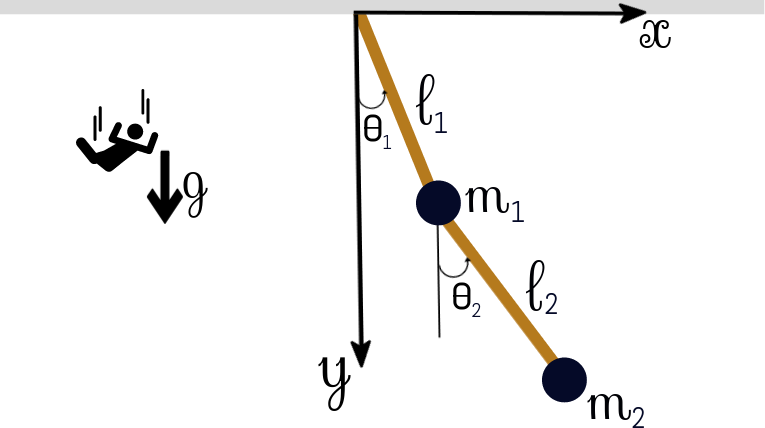
\includegraphics[scale=0.4]{problema2fig1}
\caption{Péndulo doble. Como muestra el muñequito la gravedad va dirigida hacia 
abajo.}
\label{fig:problema2fig1}
\end{figure}


Consideraremos un caso general en el cual las longitudes y masas pueden ser diferentes,
y luego haremos la simplificación que el enunciado indica. El doble péndulo consiste 
en dos masa $m_1$ y $m_2$ conectadas por barras sin masa de longitudes $l_1$ y $l_2$,
sujetas a la fuerza de gravedad, y constreñidas por las junturas entre las varas
a moverse en un plano. Escogeremos un sistema de coordenadas con el origen en el 
tope del punto de suspensión, y el eje $x$ como un eje horizontal en el plano del 
movimiento, y el eje $y$ hacia abajo, de manera tal que las fuerzas de gravedad 
tengan componentes positivas.

\section{Problema 3}

Se encuentran un compañero de la prepa que no veían desde que salieron de ella. El 
amigo estudio derecho y le ha ido muy bien; se toman un café y cuando le dicen que 
estudiaron física el se pone contento y les dice: ``que bien, mira siempre he tenido
la curiosidad de saber qué son esas cosas que ustedes tanto usan y admira: los 
tensores, dime ¿qué son?''. Escriba en media cuartilla la respuesta que le darían 
a su compañero de la prepa que estudió derecho.

\vspace{.3cm}

\underline{Solución:} \vspace{.3cm}

\section{Problema 4}

Demuestre que si la torca aplicada sobre un cuerpo rígido simétrico está a lo largo 
del eje de simetría (digamos que el eje $z$), entonces $\omega_x^2 + \omega_y^2$ es 
una constante.

\vspace{.3cm}

\underline{Solución:} \vspace{.3cm}

\section{Problema 5}

En las notas del curso se presenta una figura con la construcción de Poisont y se 
trazan las polodas, trace una figura similar en la que se muestren las herpolodas.

\vspace{.3cm}

\underline{Solución:} \vspace{.3cm}

\end{document}
